\section{Background}
\subsection{Distributed Training}
% data parallel distributed training
An ML model (e.g., neural networks, regression, support vector machine) 
consists of many parameters, and the ML training phase aims to explore the 
parameters that fit the model to the dataset. ML frameworks usually use 
gradient descending to explore such parameters.
In distributed ML training, many workers coordinate to compute the model parameters. 
One common practice is to partition the training dataset to multiple workers,
and have all workers take iterations to train the model.\footnote{One epoch has several iterations,
one iteration has several batches, and one batch trains several data points.}
In each iteration, each worker use a batch of data points (e.g., pictures in ImageNet)
to compute a gradient, all workers aggregate their local gradients and update the parameters.
In existing typical ML frameworks (e.g., TensorFlow, PyTorch\wenfei{cite}),
there are two approaches to perform the gradient aggregation and parameter update.

\textbf{(1) Parameter servers} (PS) can be deployed in the framework to aggregate the gradients 
in particular. A PS maintains a copy of parameters, receives gradients from all workers, and accumulates the gradients to the parameters (with a learning rate). If there are multiple PS'es,
each one would undertake a part of the parameters and the corresponding part of the gradient.
\textbf{(2) All Reduce} approach has workers to coordinate in a peer-to-peer way: each worker 
aggregates a part of the gradient from a few neighbors and relays the partial results to its next neighbor;
by scheduling the communication pattern (e.g., ring, binary tree), the complete result
is aggregated at one (or several workers), and broadcasted or streamed to all workers.



% two approaches

\textbf{Choice of Aggregation Approach in \sysname.} The all-reduce architecture is more suitable for 
an \emph{dedicated} infrastructure (including servers and the network) for ML applications ---
all workers coordinate in a synchronized fashion (assuming no stragglers), the
network is dedicated to the ML traffic, and the transmission protocol is scalable to the
number of workers. The PS architecture workers better in a \emph{sharing} environment
(i.e., many applications dynamically share the infrastructure) --- 
as there is a single copy of parameters at the PS, parameters are easier to be consistent
among all workers, so that stragglers and dynamic joining/leaving of workers can be tolerated
without affecting a whole ML job efficiency. In this paper, we target the multi-tenant networks
where the resources are hard to be dedicated to ML applications, so our solution would 
adopt the PS architecture.
 

\begin{table}[htb]
\caption{Compare PS and All-Reduce}
\wenfei{a tentative table}

\begin{tabular}{|c|c|c|}
\hline
\multicolumn{1}{|r|}{}         & \multicolumn{1}{r|}{\textbf{PS}} & \multicolumn{1}{r|}{\textbf{all-reduce}} \\ \hline
\textbf{asynchronzied}         & yes                              & no                                       \\ \hline
\textbf{scalability}           & no                               & yes                                      \\ \hline
\textbf{data consistency}      & yes                              & no                                       \\ \hline
\textbf{scheduling complexity} & low                              & high                                     \\ \hline
\end{tabular}
\end{table}

\subsection{In-network Computation for PS}
% advantage of in-network computation solutions
Deploying the PS architecture in the multi-tenant networks must solve the scalability issue, because 
traffic from all workers would be sent together to the PS which could easily become a bottleneck. 
In-network computation is a potential approach to solve/alleviate the scalability issue. It essential
a few network devices (i.e., programmable switches) which can perform high-speed but limited 
computation primitives on the network traffic. As the traffic traverse through the device, computation
is performed and results are carried by the traffic to end hosts. End hosts benefit from in-network 
computation by two means --- the computation is offloaded to high-speed serial processing in the 
hardware so that CPU cycles are saved and concurrency control is eliminated, and the aggregation 
computation reduces total traffic volume dramatically so that the receiver bottleneck in the 
many-to-one communication pattern can be avoided. Prototypes such as SwitchML\wenfei{cite} have
shown the acceleration of applying in-network computation in ML, storage, and communication systems \wenfei{cite}.

\begin{figure}[htb]
\centering
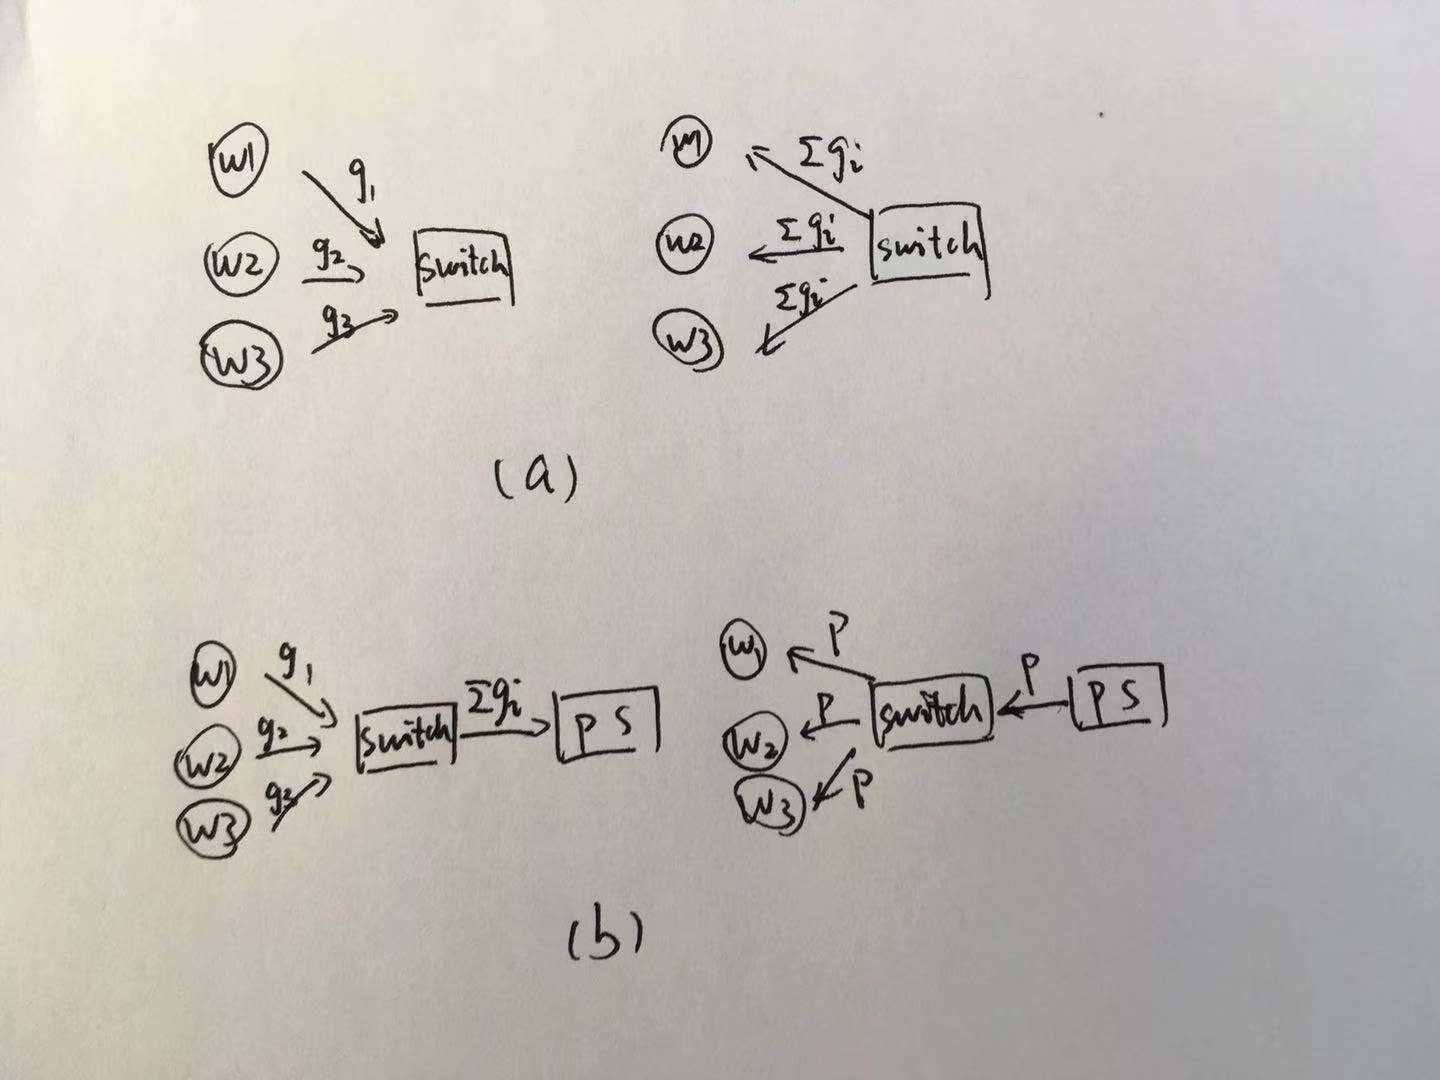
\includegraphics[width=0.8\columnwidth]{figures/strawman.jpg}
\caption{Strawman Solutions}
\end{figure}

Figure \wenfei{ref} shows two strawman solutions. In Figure Xa, the switch works as the PS --- aggregating gradients from multiple workers, and give the aggregation results back to workers; in Figure Xb, the switch performs on-path computation --- it aggregates multiple gradients and sends the result to the PS, the PS updates the parameters and reply to workers, and the switch broadcast the new parameters to the workers.

Compared with the traditional PS architecture, the bottleneck is avoided: there is no many-to-one communication pattern, avoiding overloading a specific server or network link. Compared with Ring Reduce, total network capacity (especially the number of links) and server CPU cycles 
(performing aggregation on servers) is saved.


% v.s. traditional PS
% v.s. all reduce
\subsection{Requrements for Multi-tenancy}
% requirements
Deploying an in-network computation should satisfy three basic requirements: \textbf{(R1) correctness} the computation logic should be correct without influencing the correctness of the ML application,  \textbf{(R2) performance gain} the in-network should accelerate the computation efficiency (i.e., the training speed), and \textbf{(R3) scability} the system's total processing capability should linearly increase with the number of workers. In addition, due to the nature of resource sharing in a multi-tenant network, deploying an in-network computation solution should also satisfy the following requirements.

\textbf{(R4) switch management simplicity.} In practice, the network operators build the infrastructure first, and the application developer/admin deploys the application atop the network. Thus, assuming the network should be (re)configured for applications is not practical, and any applications (including the ML application) should not complicate the switch management.

\textbf{(R5) topology freedom.} Similarly, a network topology could vary from network to network. An in-network computation solution should be deployed and work without assuming the network topology.

\textbf{(R6) ML application friendly.} While the in-network computation accelerates the communication of an ML framework, the new solution should not assume too much modification to the existing ML framework, i.e., the interfaces between the communication and computation should be kept unchanged with existing frameworks.

\textbf{(R7) Efficient Resource Sharing.} Network resources such as bandwidth and switch memory (for in-network computation) are shared among multiple ML and non-ML applications. Once contention happens, all contending applications should coverge to a stable state where network resources are efficiently used without being abused or wasted.















